\documentclass[11pt,a4paper]{article}

\usepackage{../../templates/style}

\begin{document}

\begin{problem}{Logistics}{standard input}{standard output}{1 second}{1 megabytes}

โรงงานคุโรมาตี้ (แทนด้วยตัวอักษรเอ็กซ์พิมพ์ใหญ่ ‘X’) ต้องการขนส่งสินค้าไปยังลูกค้า (แทนด้วยตัวอักษรวายพิมพ์ใหญ่ ‘Y’) ซึ่งอยู่ห่างไกล มีถนนจากโรงงานไปหาลูกค้าเพียงหนึ่งเส้น ในระหว่างเส้นทางขนส่งจะมีจุดถ่ายสินค้าอยู่ $M$ จุด $(1 \leq M \leq 26)$ แทนด้วยตัวอักษรภาษาอังกฤษพิมพ์เล็ก ‘a’ … ‘z’ เมื่อรถบรรทุกสินค้าเดินทางมาถึงจุดถ่ายสินค้าต้องขนสินค้าใส่รถคันใหม่เพื่อส่งไปยังสถานีถัดไป รถที่ประจำอยู่ที่โรงงานและแต่ละสถานีมีจำนวน $P$ คัน $(1 \leq P \leq 10)$ โดยไม่จำเป็นต้องเท่ากัน และแต่ละคันมีค่าใช้จ่ายในการขนส่งต่างกัน ยกตัวอย่างเช่น ในรูปที่ 1 จากสถานี $a$ ไปสถานี $b$ มีรถประจำสถานีอยู่ $2$ คัน $(P = 2)$ ในขณะที่จากสถานี $b$ ไปยังลูกค้า (Y) จะมีรถประจำสถานีอยู่ $3$ คัน $(P = 3)$ สำหรับรถแต่ละคันจากสถานี $a$ ไปยังสถานี $b$ มีค่าใช้จ่ายเป็น $1$ และ $4$ หน่วย

ค่าใช้จ่ายสุทธิ (Cost) ในการขนส่งสินค้าระหว่างสถานีถ่ายโอนนั้น จะมีค่าเท่ากับมัธยฐาน (Median) ของค่าใช้จ่ายของรถแต่ละคันประจำสถานีนั้น เจ้าของโรงงานจะได้รับข้อมูลค่าใช้จ่ายของรถแต่ละคัน ดังตัวอย่าง

\begin{table}[h]
\begin{center}
\begin{tabular}{|c|c|}
\hline
\centering
\begin{tabular}{lll}
X      &    a   &       1\\
a       &   X       &   7\\
a    &      b    &      4\\
b    &      a      &    1\\
b    &      Y    &      3\\
b    &     Y     &     2\\
Y     &     b   &       6
\end{tabular}% 
& 
\begin{tabular}{l}
\\
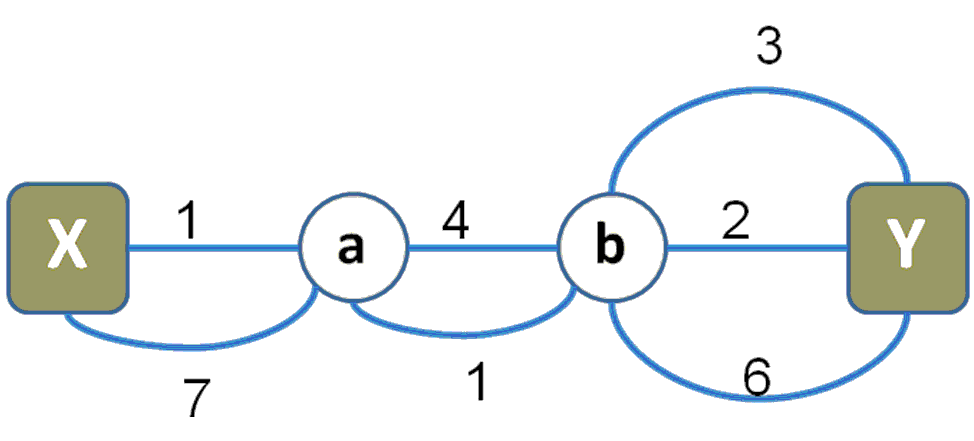
\includegraphics[width=0.4\textwidth]{../latex/img/1063/1063-1.png}\\
\end{tabular}\\
ข้อมูลค่าใช้จ่ายของรถแต่ละคันประจำสถานี & แผนผังเส้นทางและตำแหน่งของสถานีที่สมมูลกับรายงานด้านซ้ายมือ \\
\hline
\end{tabular}
\caption{ตัวอย่างข้อมูลค่าใช้จ่ายของรถแต่ละคันประจำสถานี}
\end{center}
\end{table}

จากตัวอย่างข้างต้นสามารถคำนวณค่าใช้จ่ายได้เป็นดังนี้

\begin{align}
Cost &= Median(1,7) + Median(4,1) + Median(3,2,6) \tag*{}\\
&= \frac{(1+7)}{2} + \frac{(4+1)}{2} + 3 \tag*{}\\
&= 4 + 2.5 + 3 = 9.5 \tag*{}
\end{align}

\textbf{หมายเหตุ }มัธยฐาน (\textit{Median}) เป็นค่ากลางของข้อมูล โดยพิจารณาจากข้อมูลที่เรียงแล้วจำนวน n ตัว โดยถ้ามีข้อมูลเป็นจำนวนคี่ จะเป็นข้อมูลลำดับที่ $(n+1)/2$ แต่ถ้ามีข้อมูลเป็นจำนวนคู่ จะเป็นข้อมูลค่าเฉลี่ยเลขคณิตของข้อมูลลำดับที่ $n/2$ และ $(n/2)+1$ ตัวอย่างเช่น

$Median (1, 2, 4, 3, 5)     = 3 $ \\
$Median (9, 2, 4, 5, 8, 1)  = (5 + 4)/2 = 4.5 $

\bigskip
\underline{\textbf{โจทย์}}  จงเขียนโปรแกรมเพื่อคำนวณค่าใช้จ่ายในการขนส่งสินค้าสุทธิที่เกิดขึ้น

\InputFile

\textbf{บรรทัดแรก} รับจำนวน $N$ ซึ่งแทนจำนวนรถทั้งหมดที่ใช้ในการขนส่งของทุกๆ เส้นทาง $(2 \leq N \leq 270)$

\textbf{บรรทัดที่ $2$ ถึง $N+1$} บรรทัดที่ $i+1$ รับข้อมูลของรถคันที่ $i$ โดยระบุชื่อสถานี (‘a’ … ‘z’) หรือ โรงงาน (‘X’) หรือ ลูกค้า (‘Y’) คู่ที่เส้นทางนั้นเชื่อมต่ออยู่ ตามด้วยค่าใช้จ่ายซึ่งเป็นจำนวนเต็มบวกของรถนั้นๆ $C$ $(1 \leq C \leq 20)$ (ชื่อสถานีสามารถเรียงสลับลำดับกับทิศทางของการขนส่งสินค้าจริงได้ เช่น a b และ b a หมายถึงเส้นทางเดียวกัน) โดยคั่นด้วยช่องว่าง

\OutputFile

ให้แสดงผลลัพท์ตามเงื่อนไขดังต่อไปนี้
\begin{itemize}

\item ถ้าเส้นทางขาดหาย ไม่สามารถส่งสินค้าจาก X ไป Y ได้ให้แสดง ข้อมูล\textbf{บรรทัดเดียว} ด้วยข้อความ broken
\item ในกรณีที่สามารถส่งสินค้าได้ ให้แสดง ข้อมูลส่งออกรวมทั้งสิ้น \textbf{$M+2$ บรรทัด}
ใน \textbf{$M+1$ บรรทัด}แรก แสดงเส้นทางระหว่างสถานีหนึ่งไปยังสถานีถัดไป พร้อมกับค่าใช้จ่ายของเส้นทางนั้น แสดงเป็นทศนิยมหนึ่งตำแหน่ง โดยเริ่มจาก โรงงาน X อยู่บรรทัดแรก และลูกค้า Y อยู่บรรทัดสุดท้าย
ใน\textbf{บรรทัดที่ M+2} แสดงค่าใช้จ่ายในการขนส่งสินค้าสุทธิที่เกิดขึ้น เป็นเลขจำนวนจริง ความละเอียดถึงทศนิยมหนึ่งตำแหน่ง
\end{itemize}
\Examples

\begin{example}
\exmp{6
X a 1
a b 4
b a 1
b Y 3
b Y 2
Y b 6}{X a 1.0
a b 2.5
b Y 3.0
6.5}%
\exmp{3
X a 2
c b 3
b Y 3}{broken}%
\end{example}
\begin{example}
\exmp{5
q Y 3 
X a 1
a b 2
t b 4
q t 5}{X a 1.0
a b 2.0
b t 4.0
t q 5.0
q Y 3.0
15.0}%
\end{example}


\Source

การแข่งขันคอมพิวเตอร์โอลิมปิกสอวน.ครั้งที่ 4 ปี 2551 วันที่ 2

\end{problem}

\end{document}